\chapter{Projekt systemu Team Challenge}

W niniejszym rozdziale przedstawiony został projekt systemu sporządzony na podstawie ogólnej koncepcji opisanej w poprzedniej części. W ramach projektu wydzielono role aktorów na stronie, następnie sporządzono specyfikację wymagań funkcjonalnych oraz niefunkcjonalnych. Na podstawie wymagań funkcjonalnych zostały zamodelowane encje występujące w systemie, co zostało zademonstrowane na diagramie związków encji. W ostatniej części rozdziału przedstawiono diagram stanów dla rzucanego wyzwania.

Diagramy przypadków użycia, związków encji oraz stanów zostały sporządzone przy użyciu narzędzia \textit{Visual Paradigm} w wersji 15.1. Diagram zależności między grupami w systemie uzyskano przy pomocy internetowego narzędzia \textit{draw.io}.

\section{Role w systemie}

W systemie zostały wyróżnione następujące role. 

\begin{itemize}

\item \textbf{Gość} - Niezalogowana osoba odwiedzająca system.  

\item \textbf{Użytkownik} - Zarejestrowany oraz zalogowany użytkownik systemu.

\item \textbf{Zawodnik} - Użytkownik posiadający profil zawodnika.  

\item \textbf{Kapitan} - Zawodnik, który zarządza własną drużyną. 

\item \textbf{Moderator} - Użytkownik posiadający specjalne uprawnienia. Nadzoruje jakość funkcjonalności dostarczanych przez system. Moderuje wprowadzane obiekty sportowe.    

\item \textbf{Administrator} - Specjalny użytkownik posiadający największe uprawnienia. Ma dostęp do wszystkich danych w systemie. Nadzoruje prawidłowe działanie systemu pod względem technicznym.  

\end{itemize}



\begin{figure}[H]
\centering
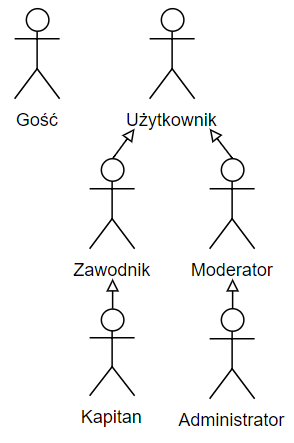
\includegraphics[width=0.5\linewidth]{04-projekt/rys/roles.PNG}
\caption{Diagram zależności między grupami w systemie}
\label{fig:diagram-groups}
\end{figure}


\section{Diagramy przypadków użycia}

Wymagania funkcjonalne zostały zdefiniowane, aby w jasny sposób opisać oczekiwania wobec systemu oraz jego zakres odpowiedzialności. Dokładne definiowanie wymagań pozwala na zidentyfikowanie możliwych błędów koncepcyjnych jeszcze przed rozpoczęciem implementacji \cite{requirements}. Specyfikacja wymagań za pomocą przypadków użycia w sposób czytelny przedstawia możliwe interakcje poszczególnych aktorów z systemem \cite{usecase}.

Poniżej przedstawiono diagramy przypadków użycia. W celu poprawienia czytelności, przypadki użycia dla niektórych aktorów zostały przedstawione na oddzielnych diagramach. 


% \subsection{Diagramy przypadków użycia}

\begin{figure}[H]
\centering
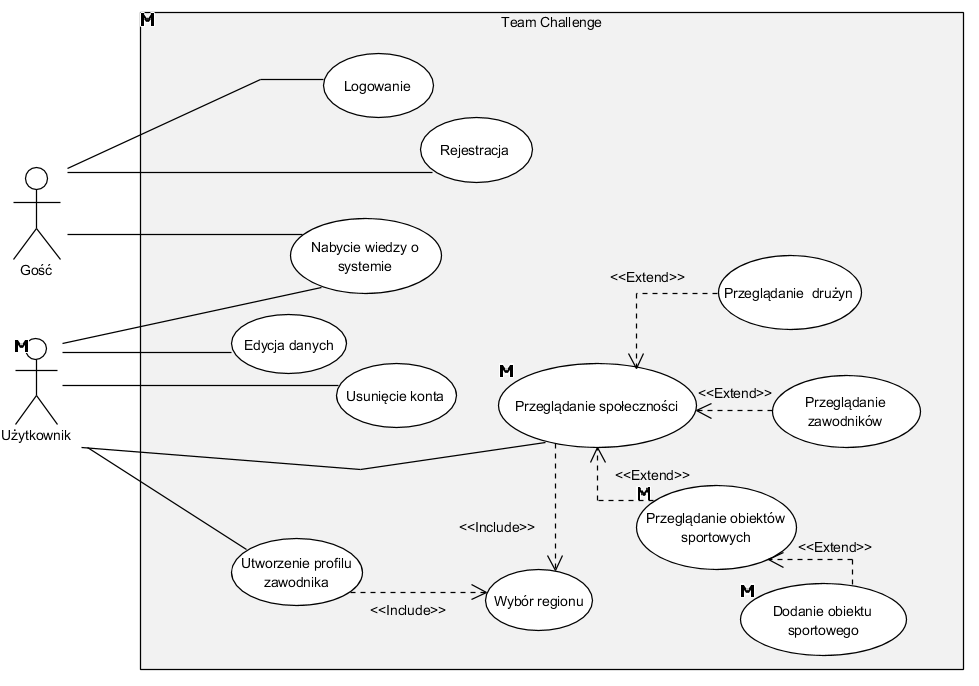
\includegraphics[width=\linewidth]{04-projekt/rys/usecase1.PNG}
\caption{Diagram przypadków użycia - gość oraz użytkownik}
\label{fig:diagram-uc-1}
\end{figure}

\begin{figure}[H]
\centering
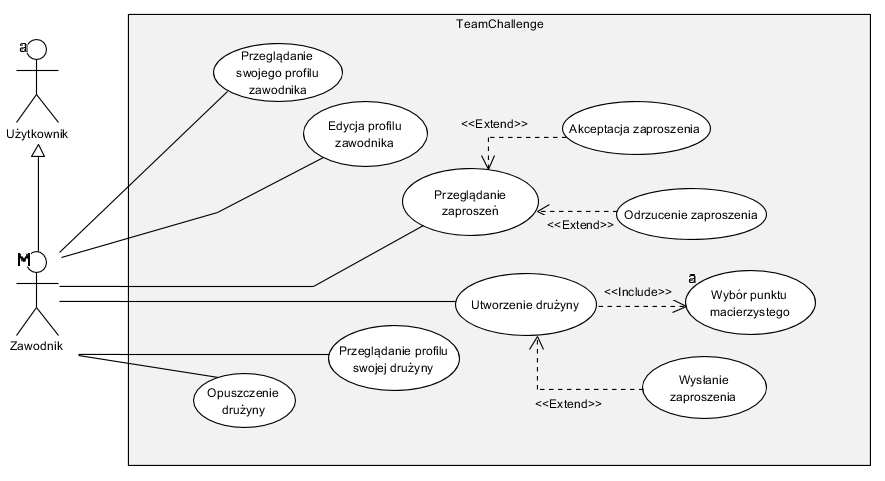
\includegraphics[width=\linewidth]{04-projekt/rys/usecase2.PNG}
\caption{Diagram przypadków użycia - zawodnik}
\label{fig:diagram-uc-2}
\end{figure}

\begin{figure}[H]
\centering
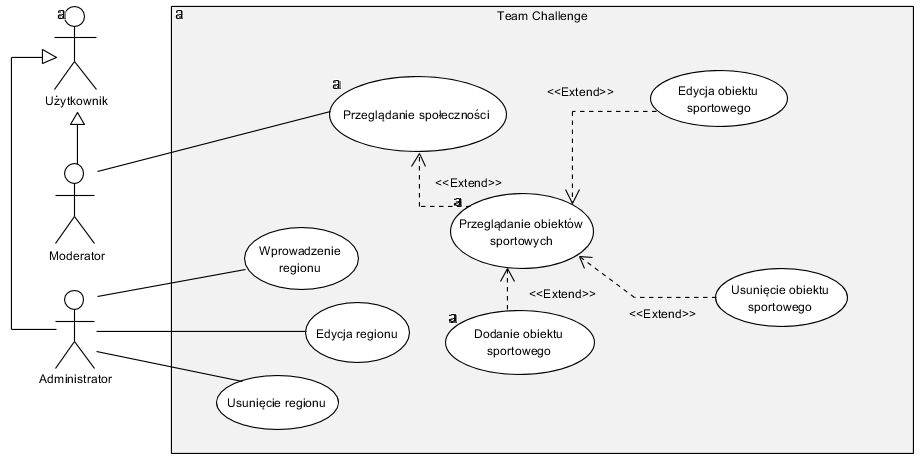
\includegraphics[width=\linewidth]{04-projekt/rys/usecase4.PNG}
\caption{Diagram przypadków użycia - moderator oraz administrator}
\label{fig:diagram-uc-3}
\end{figure}

\begin{figure}[H]
\centering
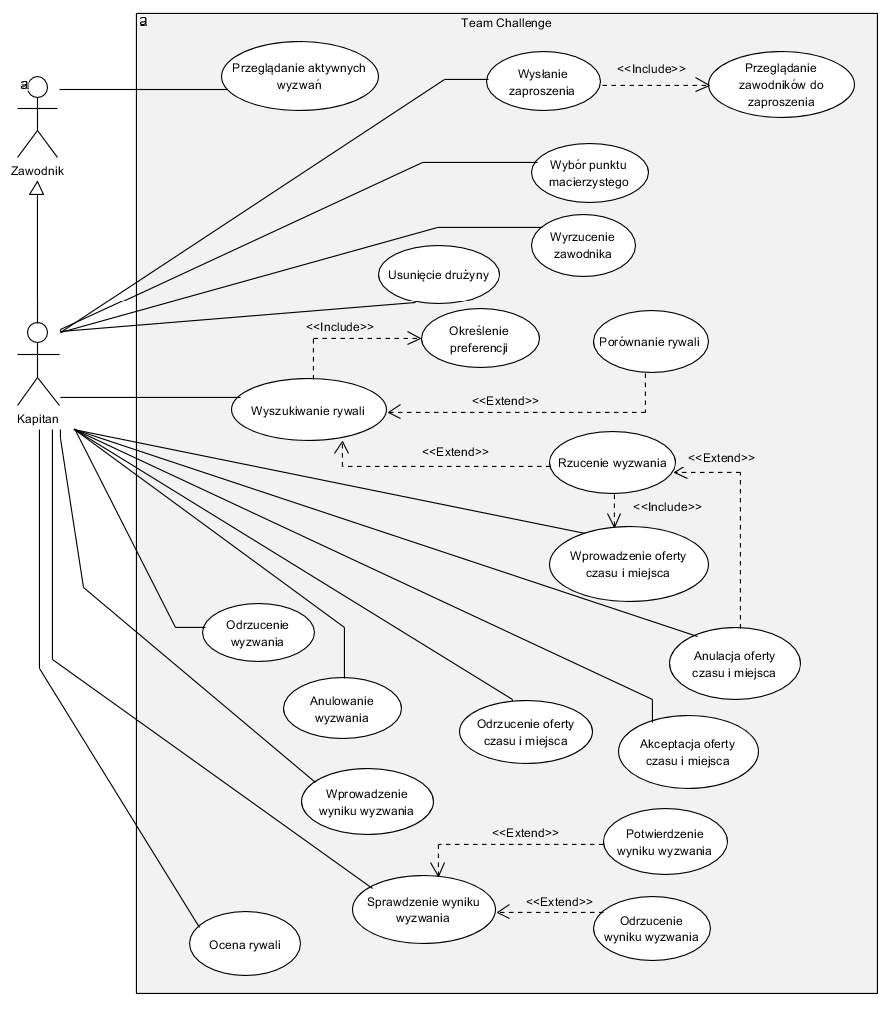
\includegraphics[width=\linewidth]{04-projekt/rys/usecase3.png}
\caption{Diagram przypadków użycia - kapitan}
\label{fig:diagram-uc-4}
\end{figure}

\section{Szczegółowe opisy przypadków użycia}

Dla wybranych spośród najbardziej istotnych przypadków użycia zostały sporządzone szczegółowe opisy zawierające warunki początkowe, końcowe oraz przebieg.

%% ------------------------ PU REJESTRACJA -------------
\subsection*{PU Rejestracja}
\subsubsection{Warunki początkowe}
Wywołanie przez gościa.
\subsubsection{Warunki końcowe}
Konto utworzone w systemie. Możliwe zalogowanie za pomocą podanego adresu e-mail oraz hasła.
\subsubsection{Przebieg}
\begin{enumerate}
  \item System wyświetla formularz rejestracyjny.
  \item Gość wypełnia formularz podając następujące dane: adres e-mail, imię i nazwisko, hasło (dwukrotnie), datę urodzenia.
  \item Użytkownik wysyła formularz za pomocą przycisku ``Zarejestruj się``.
  \begin{enumerate}[label=(\alph*)]
     \item W przypadku błędnie wypełnionego formularza system wyróżnia niepoprawnie wypełnione pola. Powrót do kroku 2.
   \end{enumerate}
  \item System zapisuje informacje o nowo zarejestrowanym użytkowniku.
  \item System informuje gościa o sukcesie oraz możliwości zalogowania.
\end{enumerate}


%% ------------------------ PU UTWORZENIE PROFILU ZAWODNIKA -
\subsection*{PU Utworzenie profilu zawodnika}

\subsubsection{Warunki początkowe}
Wywołanie przez użytkownika nie posiadającego profilu zawodnika.

\subsubsection{Warunki końcowe}
Zapisanie informacji o nowym zawodniku. Użytkownik staje się zawodnikiem oraz uzyskuje dostęp do nowych funkcjonalności.

\subsubsection{Przebieg}

\begin{enumerate}
  \item System wyświetla pierwszy krok kreatora zawodnika - podstawowe dane.
  \item Użytkownik wybiera region, w którym przebywa - wywołanie \textbf{PU Wybór regionu}.
  \item Użytkownik wprowadza swój wzrost.
  \begin{enumerate}[label=(\alph*)]
     \item W przypadku nieprawidłowej wartości system niezwłocznie informuje o tym użytkownika.
   \end{enumerate}
  \item Użytkownik przechodzi do następnego kroku kreatora za pomocą przycisku "Dalej".
  \begin{enumerate}[label=(\alph*)]
     \item W przypadku nie wypełnienia wymaganego pola dotyczącego wzrostu system informuje o tym użytkownika wyróżniając to pole. Powrót do kroku 3.
   \end{enumerate}
     
  \item System wyświetla drugi krok kreatora zawodnika - deklaracja poziomu umiejętności.
  \item Użytkownik definiuje swój poziom umiejętności dopasowując się do jednego z wymienionych oraz opisanych profili umiejętności (początkujący, średnio-zaawansowany itp.).
  \item Użytkownik określa częstość swojej gry spośród skończonej liczby możliwości przedstawionych przez system.
  \item Użytkownik tworzy profil za pomocą przycisku "Utwórz profil".
  \item System informuje użytkownika o pomyślnym utworzeniu profilu.
  \item System wyświetla użytkownikowi opcjonalny krok formularza pozwalający na wgranie zdjęcia profilowego.
 
  \begin{enumerate}[label=(\alph*)]
     \item Użytkownik może wybrać zdjęcie oraz je przesłać.
     \item Użytkownik może pominąć krok używając przycisku "Pomiń krok".
   \end{enumerate}
\end{enumerate}

%% ------------------------ PU UTWORZENIE DRUŻYNY-
\subsection*{PU Utworzenie drużyny}

\subsubsection{Warunki początkowe}
Wywołanie przez zawodnika, który nie jest członkiem żadnej drużyny.

\subsubsection{Warunki końcowe}
Zapisanie informacji o nowej drużynie w regionie zawodnika. Odrzucenie zaproszeń zawodnika do innych drużyn. Zawodnik staje się członkiem nowo utworzonej drużyny oraz jej kapitanem. Nabycie dostępu do dodatkowych funkcjonalności związanych z rolą kapitana.

\subsubsection{Przebieg}
\begin{enumerate}
  \item System wyświetla pierwszy krok kreatora drużyny - podstawowe dane.
  \item Zawodnik wprowadza nazwę drużyny.
  \begin{enumerate}[label=(\alph*)]
     \item W przypadku nieprawidłowej wartości system niezwłocznie informuje o tym zawodnika.
   \end{enumerate}
  \item Zawodnik przechodzi do następnego kroku kreatora za pomocą przycisku "Dalej".
  \begin{enumerate}[label=(\alph*)]
     \item W przypadku nie wypełnienia wymaganego pola dotyczącego nazwy drużyny system informuje o tym zawodnika wyróżniając to pole. Powrót do kroku 2.
   \end{enumerate}
   
    \item System wyświetla użytkownikowi opcjonalny krok formularza pozwalający na wgranie zdjęcia profilowego.
 
  \begin{enumerate}[label=(\alph*)]
     \item Użytkownik może wybrać zdjęcie oraz je przesłać.
     \item Użytkownik może pominąć krok używając przycisku "Pomiń krok".
   \end{enumerate}
     
  \item System wyświetla kolejny krok kreatora drużyny - wybór punktu macierzystego.
  \item Użytkownik wybiera punkt macierzysty za pomocą \textbf{PU Wybór punktu macierzystego}. A następnie potwierdza wybór za pomocą przycisku "Dalej".
  \item System informuje użytkownika o pomyślnym utworzeniu drużyny.
  \item System wyświetla użytkownikowi opcjonalny krok formularza pozwalający na zaproszenie zawodników do drużyny.
  
  \begin{enumerate}[label=(\alph*)]
     \item Użytkownik może zaprosić zawodników do drużyny - wywołanie \textbf{PU Wysłanie zaproszenia}.
   \end{enumerate}
 
\end{enumerate}


\subsection*{PU Wyszukiwanie rywali}

\subsubsection{Warunki początkowe}
Wywołanie przez kapitana, którego drużyna jest aktywna, czyli kwalifikuje się do rozgrywek. Wymogiem jest tutaj spełnienie przez drużynę warunku minimalnej liczby graczy dla danej dyscypliny.

\subsubsection{Warunki końcowe}
Prezentacja potencjalnych rywali wraz z wskaźnikami umożliwiającymi kapitanowi wnioskowanie na temat poszczególnych propozycji.

\subsubsection{Przebieg}
\begin{enumerate}
  \item Wywołanie \textbf{PU Określenie preferencji}.
  \item System na podstawie preferencji kapitana wyznacza oraz wyświetla kapitanowi listę drużyn kwalifikujących się do rozgrywek w kolejności uwarunkowanej stopniem dopasowania. Dodatkowo dla każdej propozycji system prezentuje wskaźniki pomocne w podjęciu decyzji - poziomy dopasowań poszczególnych kryteriów.
  \item Kapitan przegląda propozycje rywali.
  \begin{enumerate}[label=(\alph*)]
     \item Kapitan może porównać dwie lub trzy drużyny - wywołanie \textbf{PU Porównanie rywali}.
     \item Kapitan wnioskując na podstawie dostarczonych informacji może wybrać drużynę, której chciałby rzucić wyzwanie - wywołanie \textbf{PU Rzucenie wyzwania}.
   \end{enumerate}
   

\end{enumerate}

\subsection*{PU Określenie preferencji}

\subsubsection{Warunki początkowe}

Wywołanie z \textbf{PU Wyszukiwanie rywali}.

\subsubsection{Warunki końcowe}

System otrzymuje informacje dotyczące preferencji kapitana odnośnie poszukiwanych rywali.

\subsubsection{Przebieg}
\begin{enumerate}
  \item System wyświetla formularz deklaracji preferencji.
  \item System wyświetla podstawowe instrukcje dotyczące działania funkcjonalności.
  \item Kapitan za pomocą suwaków oraz kontrolek typu \textit{checkbox} definiuje swoje preferencje odnośnie poszczególnych cech rywali.
  \item Kapitan przesyła formularz za pomocą przycisku ``Szukaj``.
  \item System uwzględnia przesłany formularz w dalszym przetwarzaniu. 
\end{enumerate}


\subsection*{PU Rzucenie wyzwania}

\subsubsection{Warunki początkowe}

Wywołanie z \textbf{PU Wyszukiwanie rywali}. Drużyna rzucająca wyzwanie oraz wyzywana spełniają wymogi rozgrywek - są aktywne. Nie istnieje aktualne wyzwanie w toku pomiędzy tymi drużynami.

\subsubsection{Warunki końcowe}

Wyzwanie zostaje utworzone w systemie. Jest widoczne dla obydwu drużyn. Możliwe są negocjacje terminu oraz miejsca spotkania.

\subsubsection{Przebieg}

\begin{enumerate}
  \item System wyświetla podstawowe instrukcje dotyczące funkcjonalności.
  \item System wyświetla mapę, na której widoczne są punkty macierzyste drużyny kapitana oraz drużyny, której rzucane jest wyzwanie. Na mapie widoczne są również obiekty sportowe, dla których zostały utworzone oferty czasu i miejsca spotkania.
  \item System wyświetla pustą pulę ofert wraz z przyciskiem umożliwiającym dodanie oferty.
  \item Kapitan dodaje co najmniej jedną ofertę czasu i miejsca spotkania - wywołanie \textbf{PU Wprowadzenie oferty czasu i miejsca}.
  \begin{enumerate}[label=(\alph*)]
     \item Kapitan może anulować wprowadzone oferty - wywołanie \textbf{PU Anulacja oferty czasu i miejsca}.
   \end{enumerate}
  \item Gdy warunek istnienia co najmniej jednej oferty miejsca oraz czasu jest spełniony, system uaktywnia przycisk ``Rzuć wyzwanie``.
  \item Kapitan rzuca wyzwanie używając przycisku ``Rzuć wyzwanie``.
  \item System rejestruje wyzwanie w systemie, informuje użytkownika o sukcesie oraz wyświetla mu widok na którym widoczne jest utworzone wyzwanie.
\end{enumerate}

\subsection*{PU Wprowadzenie oferty czasu i miejsca}

\subsubsection{Warunki początkowe}

Wywołanie w kontekście rzucanego wyzwania bądź wyzwania będącego w trakcie negocjacji.

\subsubsection{Warunki końcowe}

Dodanie nowej propozycji czasu i miejsca spotkania do puli dla konkretnego wyzwania.

\subsubsection{Przebieg}


\begin{enumerate}
  \item System wyświetla mapę, na której widoczne są punkty macierzyste obydwu drużyn biorących udział w wyzwaniu oraz obiekty sportowe dla regionu, w którym istnieją drużyny.
  \item System wyświetla odpowiedni formularz.
  \item Kapitan wybiera datę spotkania korzystając z kalendarza. Możliwe do wyboru są jedynie daty w przyszłości.
  \item Kapitan wybiera godzinę spotkania.
  \item Kapitan wybiera miejsce spotkania wciskając wybrany znacznik obiektu sportowego na mapie.
  \item Kapitan przesyła ofertę używając przycisku "Dodaj do puli".
  \begin{enumerate}[label=(\alph*)]
     \item Kapitan może również anulować wprowadzanie oferty za pomocą\linebreak przycisku~``Anuluj``.
   \end{enumerate}
 \item System zapisuje nową ofertę oraz wyświetla kapitanowi zaktualizowaną pulę zawierającą nowo dodany element.
\end{enumerate}

\section{Wymagania niefunkcjonalne}

Po za wymaganiami funkcjonalnymi, które opisują funkcje wykonywane przez system, zdefiniowane zostały również następujące ograniczenia odnośnie procesu implementacji systemu oraz jego działania:

\begin{enumerate}

\item Zastosowane technologie muszą posiadać dokładną dokumentację techniczną.

\item Implementacja systemu musi przebiegać w sposób iteracyjny, z zastosowaniem systemu kontroli wersji.

\item Kod powstały podczas implementacji systemu powinien być czytelny oraz zrozumiały. Fragmenty mogące budzić niejasności powinny być opisane za pomocą komentarzy.

\item System powinien być szeroko dostępny. Powinien udostępniać swoje funkcje użytkownikom korzystających z różnych platform wyposażonych w przeglądarkę internetową. 

\item Interfejs systemu powinien być intuicyjny oraz prosty w obsłudze.

\item Operacje wykonywane przez system nie mogą trwać dłużej niż parę sekund. W przypadku dłuższych operacji system musi prezentować użytkownikowi ich postęp.

\item System powinien informować użytkownika o rezultatach podejmowanych akcji - sukcesach oraz błędach.

\end{enumerate}


\section{Diagram związków encji}

Na podstawie wymagań dotyczących funkcjonowania systemu zidentyfikowane zostały encje. Encje wraz ze swoimi atrybutami oraz powiązaniami zostały przedstawione w sposób graficzny na rysunku~\ref{fig:diagram-erd} za pomocą diagramu ERD (ang. \textit{Entity Relationship Diagram}).

\begin{comment}
\begin{table}[H]
\centering\small
\caption{Zestawienie encji wraz z ich opisami}
\label{tab:szablon}
\begin{tabularx}{\linewidth}{|p{.2\linewidth}|X|}\hline
Nazwa encji & Opis \\ \hline\hline

User & Dane użytkownika zarejestrowanego w systemie  \\ \hline
Authority & Poziom uprawnień użytkownika \\ \hline
GrantedAuthority & Encja pomocnicza reprezentująca uprawnienie nadane użytkownikowi \\ \hline
Discipline & Dyscyplina sportu zespołowego \\ \hline
Region & Region, w którym funkcjonuje system  \\ \hline
Position & Punkt na mapie \\ \hline
Player & Dane zawodnika\\ \hline
Team & Dane drużyny\\ \hline
TeamInvitation & Zaproszenie do drużyny wysłane przez kapitana dla zawodnika\\ \hline
Facility & Obiekt sportowy wprowadzony do systemu\\ \hline
Challenge & Wyzwanie pomiędzy dwoma drużynami\\ \hline
ChallengeStatus & Encja pomocnicza reprezentująca status wyzwania\\ \hline
PlaceTimeOffer & Oferta czasu oraz miejsca spotkania utworzona przez jedną z drużyn\\ \hline
PlaceTimeOfferStatus & Encja pomocnicza reprezentująca status oferty czasu oraz miejsca spotkania\\ \hline
Result & Wynik spotkania wprowadzony przez jedną z drużyn\\ \hline
ResultStatus & Encja pomocnicza reprezentująca status wprowadzonego wyniku spotkania\\ \hline
TeamReview & Wypełniony formularz oceny drużyny po zakończonym spotkaniu\\ \hline

\end{tabularx}
\end{table}
\end{comment}


\begin{figure}[H]
\centering
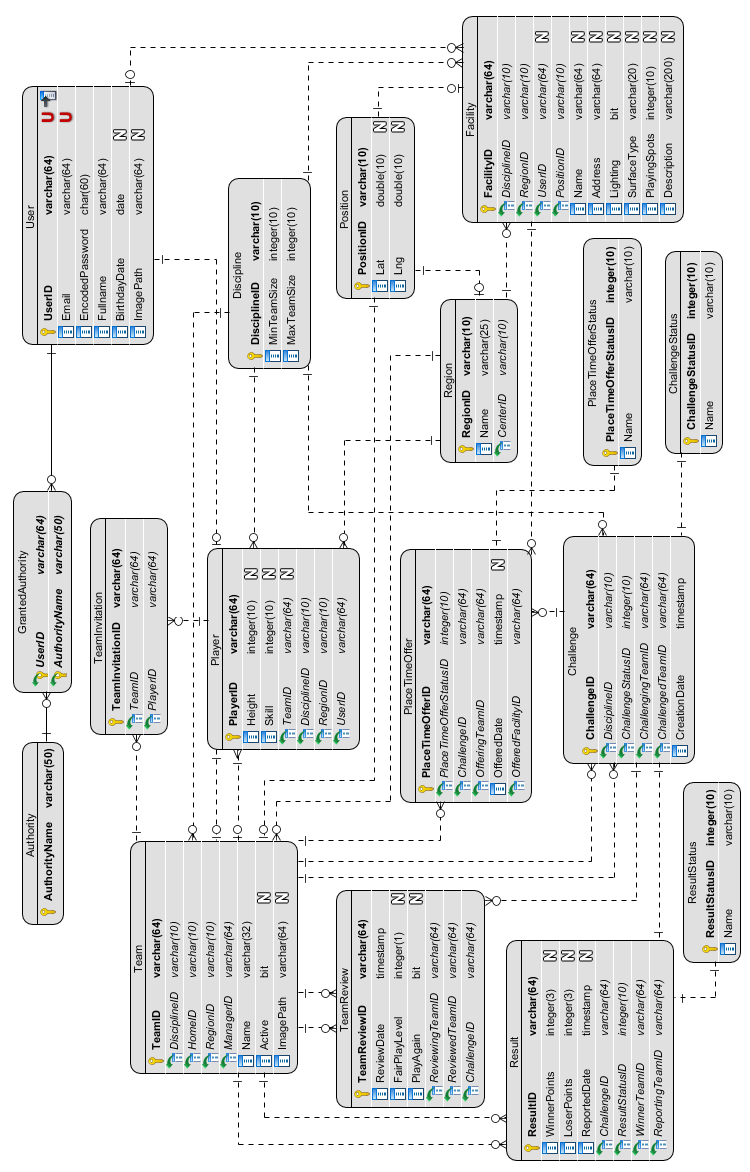
\includegraphics[width=0.85\linewidth]{04-projekt/rys/erdpoziom.PNG}
\caption{Diagram związków encji}
\label{fig:diagram-erd}
\end{figure}

\begin{comment}
\begin{figure}[H]
\centering
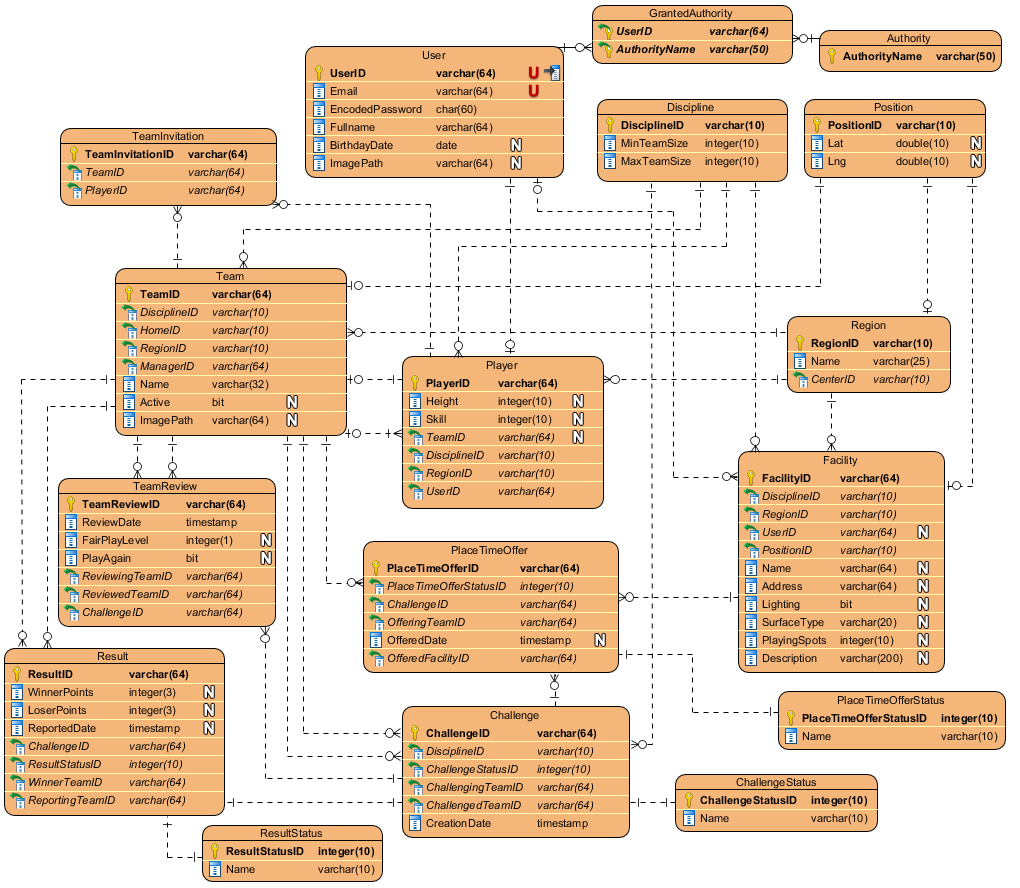
\includegraphics[width=1\linewidth]{04-projekt/rys/erd2.PNG}
\caption{Diagram związków encji}
\label{fig:diagram-erd}
\end{figure}
\end{comment}



\section{Diagram stanów - Wyzwanie}

Jedną z najważniejszych funkcjonalności systemu jest możliwość rzucania wyzwań innym drużynom. W celu ukazania możliwych stanów w jakim może znajdować się wyzwanie sporządzono diagram stanów. Diagram został przedstawiony na rysunku \ref{fig:diagram-stany-wyzwanie}. 

\begin{figure}[H]
\centering
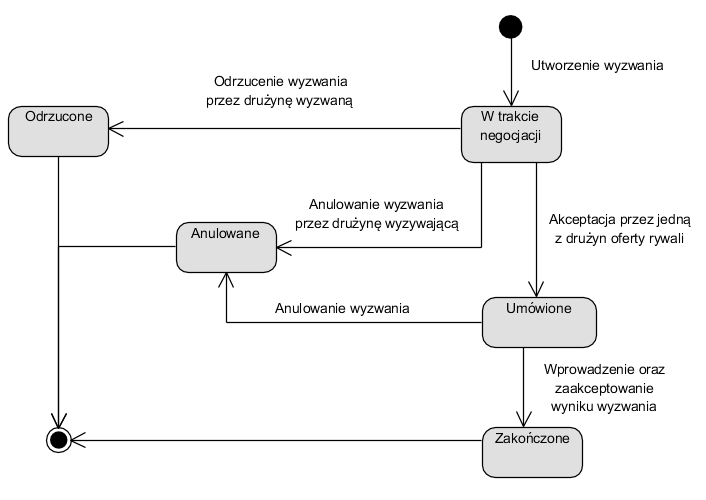
\includegraphics[width=0.8\linewidth]{04-projekt/rys/state1.PNG}
\caption{Diagram możliwych stanów wyzwań}
\label{fig:diagram-stany-wyzwanie}
\end{figure}



